\documentclass{article}
\usepackage[UTF8]{ctex}
\usepackage{amsmath,mathtools,geometry,pgfplots,float,mathrsfs,caption}
\pgfplotsset{compat=1.15}
\usetikzlibrary{arrows}
\geometry{scale=0.7}

\title{每日一题(15.2)}
\author{\kaishu 李东宸、程昊一}
\date{2022年4月20日}

\begin{document}
\maketitle
\textbf{1. }如图, 已知$BO=2DO$, $CO=5AO$, 阴影部分面积的和为11, 求$\mathrm{S}_{\text{四边形}ABCD}$.\\
\rightline{\kaishu(李东宸供题)}
\begin{figure}[H]
	\flushright
	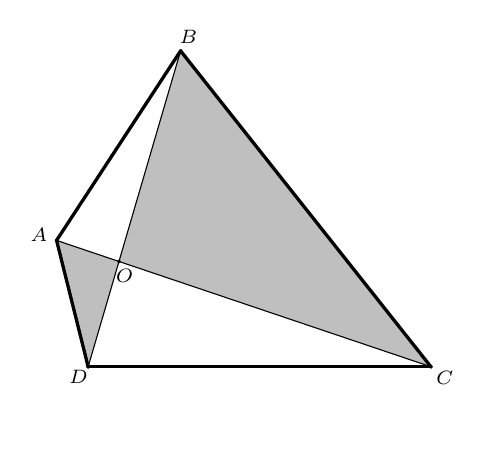
\begin{tikzpicture}[line cap=round,line join=round,>=triangle 45,x=1.0cm,y=1.0cm]
		\clip(-0.367008024670935,-0.8033932337294809) rectangle (5.072454015088062,4.306259354055769);
		\fill[line width=2.pt,fill=black,fill opacity=0.25] (0.792362860281431,1.337133023001143) -- (0.,1.6045596276013714) -- (0.40101,0.) -- cycle;
		\fill[line width=2.pt,fill=black,fill opacity=0.25] (0.792362860281431,1.337133023001143) -- (1.575068580844293,4.01139906900343) -- (4.754177161688586,0.) -- cycle;
		\draw [line width=1.2pt] (0.,1.6045596276013714)-- (0.40101,0.);
		\draw [line width=0.4pt] (0.,1.6045596276013714)-- (4.754177161688586,0.);
		\draw [line width=1.2pt] (4.754177161688586,0.)-- (0.40101,0.);
		\draw [line width=1.2pt] (1.575068580844293,4.01139906900343)-- (0.,1.6045596276013714);
		\draw [line width=1.2pt] (1.575068580844293,4.01139906900343)-- (4.754177161688586,0.);
		\draw [line width=0.4pt] (1.575068580844293,4.01139906900343)-- (0.40101,0.);
		\begin{scriptsize}
			\draw [fill=black] (0.,1.6045596276013714) circle (0.5pt);
			\draw[color=black] (-0.22345109898504092,1.6778044391505802) node {$A$};
			\draw [fill=black] (0.40101,0.) circle (0.5pt);
			\draw[color=black] (0.2768135534844053,-0.13349861289396037) node {$D$};
			\draw [fill=black] (4.754177161688586,0.) circle (0.5pt);
			\draw[color=black] (4.9286998046083355,-0.13924878131314938) node {$C$};
			\draw [fill=black] (0.792362860281431,1.337133023001143) circle (0.5pt);
			\draw[color=black] (0.863330732241687,1.1602892814235686) node {$O$};
			\draw [fill=black] (1.575068580844293,4.01139906900343) circle (0.5pt);
			\draw[color=black] (1.6741044793473412,4.190628038336182) node {$B$};
		\end{scriptsize}
	\end{tikzpicture}
\end{figure}\par
\vspace*{-1cm}\textbf{2. }如图, $ABCD$为正方形, $M$, $N$为$AB$的三等分点, $P$为$BC$中点, 求$\mathrm{S}_{\text{四边形}MNTS}$.\\
\rightline{\kaishu (程昊一供题)}
\begin{figure}[H]
	\flushright
	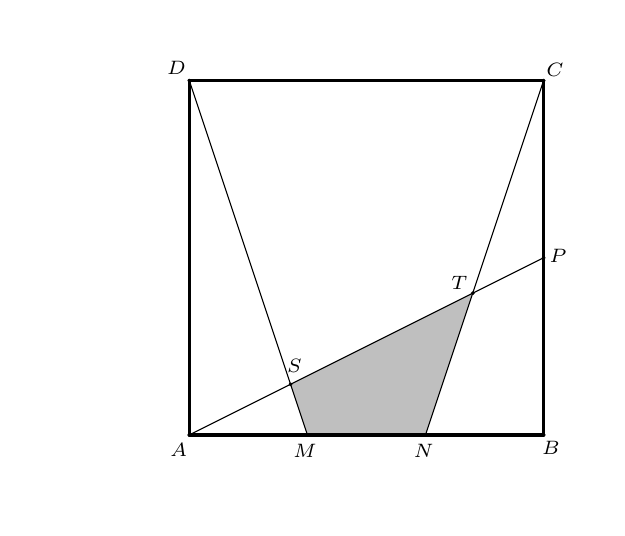
\begin{tikzpicture}[line cap=round,line join=round,>=triangle 45,x=1.5cm,y=1.5cm]
		\clip(-1.3684913149744464,-0.6138736113254375) rectangle (3.453719962736984,3.447860636177753);
		\fill[line width=2.pt,fill=black,fill opacity=0.25] (0.8571428571428571,0.42857142857142855) -- (1.,0.) -- (2.,0.) -- (2.4,1.2) -- cycle;
		\draw [line width=1.2pt] (0.,0.)-- (3.,0.);
		\draw [line width=1.2pt] (3.,0.)-- (3.,3.);
		\draw [line width=1.2pt] (3.,3.)-- (0.,3.);
		\draw [line width=1.2pt] (0.,3.)-- (0.,0.);
		\draw [line width=0.4pt] (1.,0.)-- (0.,3.);
		\draw [line width=0.4pt] (2.,0.)-- (3.,3.);
		\draw [line width=0.4pt] (3.,1.5)-- (0.,0.);
		\begin{scriptsize}
			\draw [fill=black] (0.,0.) circle (0.5pt);
			\draw[color=black] (-0.08903026053639303,-0.12701986450802005) node {$A$};
			\draw [fill=black] (3.,0.) circle (0.5pt);
			\draw[color=black] (3.0625833662044,-0.11290816170171811) node {$B$};
			\draw [fill=black] (3.,3.) circle (0.5pt);
			\draw[color=black] (3.0955106727524386,3.0904483753288257) node {$C$};
			\draw [fill=black] (0.,3.) circle (0.5pt);
			\draw[color=black] (-0.10784586427812912,3.109263979070562) node {$D$};
			\draw [fill=black] (1.,0.) circle (0.5pt);
			\draw[color=black] (0.9787552518071294,-0.13172376544345404) node {$M$};
			\draw [fill=black] (2.,0.) circle (0.5pt);
			\draw[color=black] (1.9853900519900096,-0.13290816170171811) node {$N$};
			\draw [fill=black] (3.,1.5) circle (0.5pt);
			\draw[color=black] (3.1237340783650427,1.5146415619584408) node {$P$};
			\draw [fill=black] (0.8571428571428571,0.42857142857142855) circle (0.5pt);
			\draw[color=black] (0.8893811340338831,0.5832691767425117) node {$S$};
			\draw [fill=black] (2.4,1.2) circle (0.5pt);
			\draw[color=black] (2.286439711857787,1.2888543170576094) node {$T$};
		\end{scriptsize}
	\end{tikzpicture}
\end{figure}
\end{document}